\chapter{Discussion}
\label{cha:discussion}

\section{Evaluation}
\label{sec:evaluation}

\begin{comment}
When evaluating your results, avoid drawing grand conclusions, beyond those that your results can in fact support.
Further, although you may have designed your experiments to answer certain questions,
the results may raise other questions in the eyes of the reader.
It is important that you study the graphs/tables to look for unusual features/entries, and discuss these as well as the main findings.
In particular, carry out an error analysis: What went wrong and why?

A confusion matrix can, for example, be a good way to display misclassifications.
Figure~\ref{fig:conf_sentiment} (on Page~\pageref{fig:conf_sentiment}) shows two confusion matrices.
If there were perfect correlation between true and predicted labels, the long diagonals (from the upper left to the lower right corner) would be completely red.
However,  the confusion matrices indicate
that this classifier was quite biased towards the neutral label (illustrated with \Neutrey),
as can be seen from the warm colours in the positive (\Smiley) and negative (\Sadey) true label cells of the \Neutrey predicted label column.

% Axis configuration for confusion matrices with pgfplots
\pgfplotsset{
    colormap={whitehot}{color(0cm)=(white); color(1cm)=(yellow); color(2cm)=(orange); color(3cm)=(red)},
    confusionaxis/.style={
            colorbar,
            colorbar style={
                    width=2mm,
                    at={(1.05,1)},
                },
            colormap name=whitehot,
            faceted color=none, % remove lines between fields
            view={0}{90},
            y dir=reverse,
            xlabel=Predicted label,
            ylabel=True label,
            tick style={draw=none},
            yticklabels={,,},
            xticklabels={,,},
            every node=[font=\small],
            extra x ticks={0.4,1.5,2.6},
            extra x tick labels={\Smiley, \Neutrey, \Sadey},
            extra y ticks={0.3,1.5,2.7},
            extra y tick labels={\Smiley, \Neutrey, \Sadey},
            extra x tick style={
                    x tick label style={
                            font=\Large
                        }
                },
            extra y tick style={
                    y tick label style={
                            font=\Large
                        }
                },
            width=.4\linewidth,
        }
}

\begin{figure}[t!]
    \centering
    \begin{subfigure}{\linewidth}
        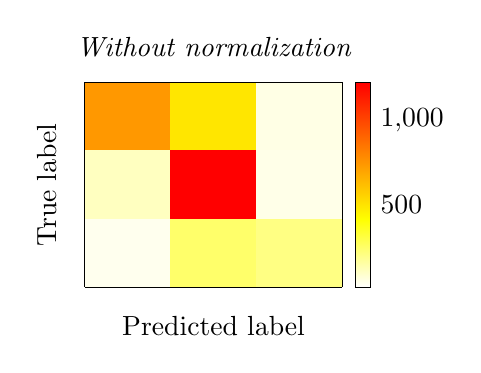
\begin{tikzpicture}
            \begin{axis}[
                    confusionaxis,
                    title={\em Without normalization},
                ]
                \addplot3
                [surf,mesh/cols=4,shader=flat corner
                ] coordinates {
                        (0,0,740) (1,0,490 ) (2,0,43 ) (3,0,1)
                        (0,1,102) (1,1,1229) (2,1,38 ) (3,1,1)
                        (0,2,28 ) (1,2,240 ) (2,2,199) (3,2,1)
                        (0,3,1  ) (1,3,1   ) (2,3,1  ) (3,3,1)
                    };
            \end{axis}
        \end{tikzpicture}
        %\hfill
        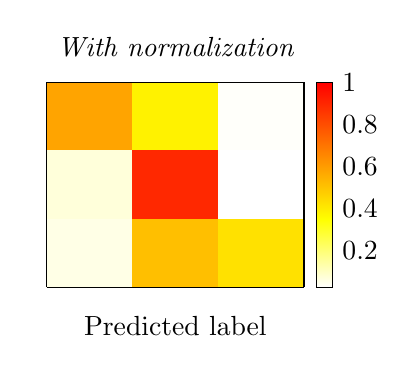
\begin{tikzpicture}
            \begin{axis}[
                    confusionaxis,
                    title={\em With normalization},
                    ylabel={},
                    colorbar style={
                            ylabel={},
                            yticklabel style={
                                    align=right,
                                }
                        },
                ]
                \addplot3
                [surf,mesh/cols=4,shader=flat corner
                ] coordinates {
                        (0,0,0.58130401) (1,0,0.38491752) (2,0,0.03377848) (3,0,1)
                        (0,1,0.07450694) (1,1,0.89773557) (2,1,0.02775749) (3,1,1)
                        (0,2,0.05995717) (1,2,0.51391863) (2,2,0.4261242 ) (3,2,1)
                        (0,3,1         ) (1,3,1         ) (2,3,1         ) (3,3,1)
                    };
            \end{axis}
        \end{tikzpicture}
        \label{fig:conf_sentiment_2013}
    \end{subfigure}
    \caption{Sentiment classifier confusion matrices}
    \label{fig:conf_sentiment}
\end{figure}
\end{comment}

\section{Discussion}
\label{sec:discussion}

\begin{comment}
In this section it is important to include a discussion of not just the merits of the work conducted, but also the limitations.
Which choices did you make? Why? What alternatives were there?
{\color{red}\textbf{Note that a key part of the Master's Thesis grading is based on the student's ability to discuss the results in light of the work by others as well as the restrictions and potential of the work itself.}}
While the Results section will report the outcome of each specific experiments, the Discussion should put those results into perspective and look at overall lessons that can be learned from the entire series of experiments.

You should be able to discuss your work in relation to its overall goal and your research questions (i.e., those introduced in Chapter~\ref{cha:introduction}),
but also address issues such as any ethical considerations that the work may entail,
as well as its technical challenges and limitations.

Discussion and evaluation can either be two different chapters, a joint chapter (as here), or part of the concluding chapter
--- or the discussion can be part of that chapter while the evaluation is part of the experimental chapter.

As for most parts of the thesis, it is possible to select various outlines and setups for the discussion; the important thing is that all the relevant parts appear \textit{somewhere\/} in the text.
\end{comment}

\cite{yiuTransmissionTruthImitation2023} calls \acrshort{acr:ai} technologies like \acrlongpl{acr:llm} "powerful imitation engines" but claim that they are unable to innovate and that significant advancements in \acrshort{acr:ai} development is required for them to be able to learn the in the same way human children do.

\subsection{Using the In-Built ChatGPT Code Interpreter for Geospatial Analysis}

When using ChatGPT's Code Interpreter with file uploads, it became apparent that it runs in a Linux environment, and that it uses a mounted drive  in the \texttt{/mnt} director, which is used for temporarily mounted filesystems. From the initial experiments where the same data in different file formats was tested it tried to a \acrshort{acr:gdal} command (\texttt{ogr2ogr -f "GeoJSON" \{converted\_geojson\_path\} \{sosi\_file\_path\}}) to perform a conversion from \acrshort{acr:sosi} to GeoJSON, the latter of which is far easier to manipulate in a Python environment. This test failed, and the system's response was that \enquote{the \texttt{ogr2ogr} tool is not available in this environment}.

This result was not very surprising, especially since the driver needed to read and write \acrshort{acr:sosi} files---which is called \textit{fyba} and is developed by The Norwegian Mapping Authority\footnote{\url{https://github.com/kartverket/fyba}}---is almost certaintly not available in the standard Linux environment for ChatGPT's Code Interpreter. Seeing as the \acrshort{acr:sosi} standard still is widely used for Norwegian geospatial purposes (though expected to be exchanged with the \acrshort{acr:gml} format in the future), it is important for an \acrshort{acr:llm}-based \acrshort{acr:gis} agent focused on the Norwegian market to be able to handle this file type.

The inability to manipulate the Linux environment using by the Code Interpreter clearly poses some limitations on the systems. A solution to the problem is to create a custom environment on a server and implement agent-like capabilities by other means (LangChain, AutoGPT, AutoGen, etc.). Having the agent run on an environment that we control ourselves gives us greater flexibility, and we can then allow the agent to access powerful \acrshort{acr:gis} tooling, such as the \acrshort{acr:gdal} library. This also allows us to avoid having to perform I/O on a mounted directory (in the \texttt{/mnt} directory), which can increase the speed of reads and writes.

\glsaddall